\section{Research Method}

This study follows the guidelines for design research in information systems, as presented by~\cite{Hevner2004}. % \todo{(Vaishnavi \& Kuechler, 2004)}. 
In this section we describe the steps we followed in order to propose our suggestion and collect feedback. 

In summary, the steps we followed were as follows: 
 \begin{enumerate}
  \item Understand the context of the problem by performing semi-structured interviews and code analysis.
  \item Capture, document and analyze the extracted information.
%  \item Perform literature review to explore available solutions from the state of the art.
  \item Provide trade-off analysis for each variability point.
  \item Conceive a solution and realize a prototype for showing the idea.
  \item Evaluate by collecting feedback from key stakeholders in the company
  \item Iterate this process, refine the method, expand the scope and re-evaluate
 \end{enumerate}

%\subsection{Research Method}
We first had to understand the context of the problem. Then, we explored the current available solutions and select the optimum by providing the reasoning behind. This enabled us to suggest a way to solve it by designing a prototype. We then proceeded to evaluate our suggestion based on the feedback of the company's stakeholders. Based on that we further refined our method. Additionally,  to assess whether or not our approach could be applied to another similar context, we used the findings of the first iteration to suggest a way for another interface. Feedback from experts was once again collected and documented. 

%Figure~\ref{fig:method} shows the process steps we followed.
%
%\begin{figure}[h]
%\centering
%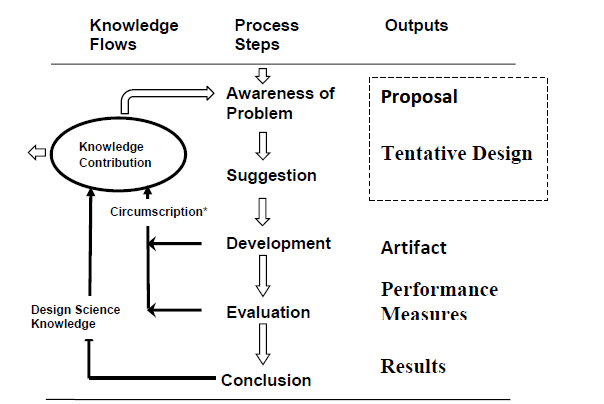
\includegraphics[width=\columnwidth]{figure/Figure1.png}
%\caption{The process model for design research. Taken from~\cite{Hevner2004}}
%\label{fig:method}
%\end{figure}


%
%\subsection{Awareness of the problem}
%Initially, the focus was placed on the SSIM interface only. After concluding the first iteration with the evaluation we decided to expand the scope to a second interface. Due to time constrains and the required effort to build the required components, the second iteration had a more theoretical approach.  
%\subsubsection{Interviews}

\noindent {\bf Awareness of the problem:} In an attempt to extract the knowledge which was dispersed in several stakeholders of the company, we conducted a number of semi-structured interviews. In this way, we gained an insight about the context of the SSIM interface, the customization procedures and other relevant technical information. The identification of right interviewees was considered fundamental for the study. %We wanted to extract as much relevant information as possible. 
For this reason we focused on stakeholders who worked with interfaces, either as developers or by interacting with customers. %Some interviewees had a hard time to give us relevant information that we needed but they helped us by pointing some other person who could help us more during our analysis phase. 
%We only kept the information we believed was relevant for our study, after the interviews were complete. Irrelevant information for example could be about the difficulty to understand error reports when the parsing of SSIM files fail, as it had nothing to do with improving the customization of this interface.
Those stakeholders were in total twelve, as shown in Table~\ref{tab:stakeholders}. 

 
%\begin{itemize}
%\item
%% Hokan
%A developer who worked in the implementation of the SSIM parser in the old system.
%
%\item
%%anton, phillipe, camtcha 
%Three software engineers involved in the development of the new system, including the SSIM parser.
%%Robert
%\item A system's expert involved in the production of the new system who also gave us an insight of the new system's architecture.
%
%%Thekla
%\item A system Architects of the Core Technical Development, involved in the development of the old system but also provides support in the new system's architecture.
%
%%IO product owner
%\item A process consultant who also plays the role of the Product Owner of the new system.
%
%%Stefan
%\item A system expert who is also a Subject Matter Expert in pairing systems and with vast experience in the old system.
%%Henrik Magnus
%\item Two service managers from the Service center, who come in contact with clients.
%%Hans Andreason
%\item A systems expert from the Implementation Department, who engage in customization and delivery procedures, sometimes with the help of customers.
%%Hans Eriksson
%\item A Business Consultant involved in premarket and benchmark activities
%
%\end{itemize}
%%\hfill 

\begin{table}[h]
\begin{center}
{\small 
\begin{tabular}{|p{.15cm}|p{1.3cm}|p{5.5cm}|}
\hline\hline
{\bf \#} & {\bf Role} & {\bf Reason/Expertise}\\
\hline
1 & Developer & Worked in the implementation of the SSIM parser in the old system\\
\hline
3 & Software engineer & Involved in the development of the new system, including the SSIM parser\\
\hline
1 & System expert & Involved in the production of the new system who also gave us an insight of the new system's architecture\\
\hline
1 & System architect & Part of the core technical development, involved in the development of the old system, provides support in the new system's architecture\\
\hline 
1 & Process consultant & Plays the role of the product owner of the new system\\
\hline
1 & System expert & Subject Matter Expert in pairing systems and with vast experience in the old system\\
\hline
2 & Service manager & Contact person with clients\\
\hline
1 & Systems expert  & Part of the implementation department and engages in customization and delivery procedures, sometimes with the help of customers\\
\hline
1 & Business Consultant & Involved in premarket and benchmark activities\\
\hline\hline
\end{tabular}}
\end{center}
\caption{Interviewed stakeholders}
\label{tab:stakeholders}
\end{table}


%The interviews followed a semi-structured approach by preparing questions beforehand. 
Each interview was planned for at least thirty minutes. However, some of the interviews took longer, with a maximum time of one hour and twenty minutes, as we allowed the interviewees to elaborate more based on topics that were considered relevant to the study. 
All the interviews were recorded and later transcribed for further analysis. 

Additionally, in an attempt to mitigate the risk that we might have missed some important aspect or that the questions might have been misunderstood by the experts and also to ensure the consistency of our findings a group interview also took place. In the group interview engineers from both the new and old system were involved and we allowed them to discuss with each other for each point that was raised. The total time of the group interview was approximately sixty minutes.

The main focus of all interviews was placed on identifying the variability issues within the SSIM interface. However, to further facilitate our understanding of the general context that this interface operates in, other issues were also taken into consideration. Discussion about the high-level architecture of the new system as well as the general demonstrations of the company's business goals and challenges took place during this phase.

%\subsubsection{Code and document analysis}
\noindent {\bf Code and document analysis:} 
In addition to the interviews we performed also an analysis in deep of the code and of the available documentation. 
The aim of this study is to allow the new system's integrator to become more configurable. We therefore considered code analysis of both the old and the new system's source code as an essential part of our study. Main focus was placed on the translation process of the SSIM files, containing raw data, to semantics which the company's system can understand. We analyzed the code both of the old and the new system. Especially in the new system, code analysis was essential for the development of the prototype as it required understanding of the classes, their methods, their data structures and their dependencies. 

For the code analysis of the old system an engineer who had worked a lot on the SSIM integration part was also involved. We used screen capturing software to record the code analysis in order to facilitate its documentation. In this way we could look into the code multiple time with the expert's commentary and grasp the issues of the old approach. He explained how the code was written and refactored in the past, the challenges they have faced and the causes of complexity. Moreover he proceed to demonstrate the functionality of the system by running some test cases. 

The code analysis of the new system was mostly done manually by us. However, support of the engineers was provided by answering our questions and providing short explanation of the reasoning behind their implementation. We have also been involved in the new system's team meetings where we kept notes of their discussions. These meetings discussed mostly the architectural aspects of the new system's integrator. 
%Finally, analysis of relevant company documentation was applied. 

These documents included the 2011 version of the IATA standard manual, architecture diagrams, official manuals and tutorials of both systems. Especially the manual of the IATA standard helped us a lot to understand the code of both systems and based on that we got a grasp of the customer specific use cases that have appeared in the past or might appear in the future.


%\subsection{Literature review}
%In order to get a background of the research problem, a set of research papers, journal articles and dissertations have been selected. The core focus was placed on the variability
%management and handling, software customization and design patterns. Our purpose is to adopt a method based on the state-of-the-art variability handling methods which we consider relevant to the company's technical context. In the previous chapter we discussed the related work based on the literature review. 
%We started by reviewing a systematic literature about variability in software systems done by (Galster et al. 2014). We read the summary of variability mechanisms in product lines by (Lee \& Hwang 2014) and also reviewed the referenced papers. We adopted definitions presented in (Svahnberg, van Gurp \& Bosch, 2001), a paper which is cited many times. We also followed their taxonomy for variability realization techniques in (Svahnberg, van Gurp \& Bosch, 2005) which is also referenced by many other papers. 
%The keywords we used to obtain references from various digital libraries were closely related to variability management. Literature related to variation point models, patterns for software variability, variability modelling and software customization were selected. The appropriateness of the selected literature is evaluated by
%reading the abstract and introduction, the proposed tools and frameworks and their implementation or the overview of the method and finally the conclusion of the study.
%In the related work chapter we presented the main methods we discovered. 

%\subsection
\noindent {\bf Trade off analysis and development}: 
%blabla gia trade off. 
We were looking for a solution which would adhere to the requirements of the company's stakeholders. We therefore wanted a solution with as minimal effort to implement as possible. During the trade off analysis we looked through the available methods in the literature; we assessed their applicability on the company's context and their expected strengths and weaknesses. 
We documented the results of the analysis and discussed the different methods with stakeholders in the company. Based on their feedback we decided which of the methods were more appropriate for interface customization and we proceeded to develop a prototype. 
In section~\ref{sec:approach} we present the trade off analysis for each method. 

%\subsection{Development}

%Having concluded with the trade off analysis, we picked a method and went on to design a prototype. The initial design was on the core Java implementation. However, when the company changed to Python, we went a step back and tried another approach. 

%The idea was to observe whether or not we could support the customization of the use cases we found through the interviews. Each use case was dealt in isolation and we observed whether or not our suggestion could support them.
\noindent {\bf Solution construction}: 
Having concluded with the trade off analysis, we picked a method and went on to design a prototype. The idea was to observe whether or not we could support the customization of the use cases we found through the interviews. Each use case was dealt in isolation and we observed whether or not our suggestion could support them. 
The development was done in a test-driven development approach. We started by writing a test case which represented a use case and let it fail. We then wrote code which would make the test case pass. The prototype included a separate python module which would inherit and overwrite parts of the system's core code. The core code was left intact. 



%\subsection{Evaluation}
\noindent {\bf Evaluation}: 
After the completion of the prototype we proceeded to evaluate it. We wanted to get early feedback to see whether or not our method is aligned with the company's customization needs so as to decide how we would continue.  For this purpose, we invited experts from the company to collect initial feedback. The stakeholders involved were a system expert of the new system and a service manager from the service center department. The system expert was the person who wrote the parser's code in Python. The person from the service center was selected because he comes in contact with customers. 

The evaluation started by asking permission to record the evaluation. We later used slides and performed a live demonstration of our prototype. We asked their opinion of the strengths and weaknesses of our approach. We transcribed and analyzed their feedback. Based on it we would then proceed to refine our method further. 

The final evaluation took place after the refinement of our original approach. The stakeholders involved were engineers of the new system, one of the new system's architect, an architect from the core development product, a line manager and a stakeholder from the implementation team. The presentation included slides which gave an overview of our work, the problem at hand and the flow of logic of how we concluded to our results. After the presentation we encouraged the employees to give us their opinion. We stressed the importance of why they think this way. We encouraged them to elaborate on the reason they think our approach is good or bad and to discuss with each other.


\section{Towards effective variability handling}\label{sec:approach}


The first step towards an effective way to handle variability is by understanding it. This is also required if we want to answer the first research question regarding the variability needs and limitations. For each variability point, we identify the variable item, why different airlines have different needs and which are the required variants, as suggested by~\cite{Pohl2005}. % (Pohl, B�ckle,  Linden. 2005 p60). 

In this section we present the main variation points of SSIM and Operational Messages interfaces. We then present an overview of how the old and the new system parse SSIM files. Finally, we discuss the indicators which influenced our decision making and provide a trade-off analysis of variability realization mechanisms.


\subsection{Variation inside standard interfaces}
\subsubsection{Main Variation Points of SSIM}

The results of the analysis phase led to the identification and grouping of the main variation points of the investigated interface. We use the term variation point to describe the parts of the standard which are open for interpretation from customer to customer. The system needs to be aware of these fields and their required variants, providing a mechanism to handle the possible use cases. 

Some of the issues of more technical nature were not considered as variation points. These issues were mainly related with the inability of some customers to produce proper SSIM files complying with the IATA standard. For example, a customer might include four bytes in a field that is meant to contain only two, ruining the syntax for the rest of the fields. It is then up to the customer to fix the syntax of the corrupted files and resend it again. 
%pes oti eixame provlima na kanoume extract ta UC

During our interviews we observed that the various stakeholders had some difficulty to remember all the use cases which appeared in the past. During the group interview, the significance of each variation point was discussed. The general feeling was that the standard should be the same for everyone and there should be no room for interpretation. However some stakeholders strongly believe that this can hardly be the case and it is very likely that airlines will impose their own use cases, as it happened before. By the time our study started, the new system was supporting only one customer and the requirements for the next ones were not known. 


We summarize the main variation points of the SSIM in Figure~\ref{fig:SSIMvariability}.

\begin{figure}[h]
\centering
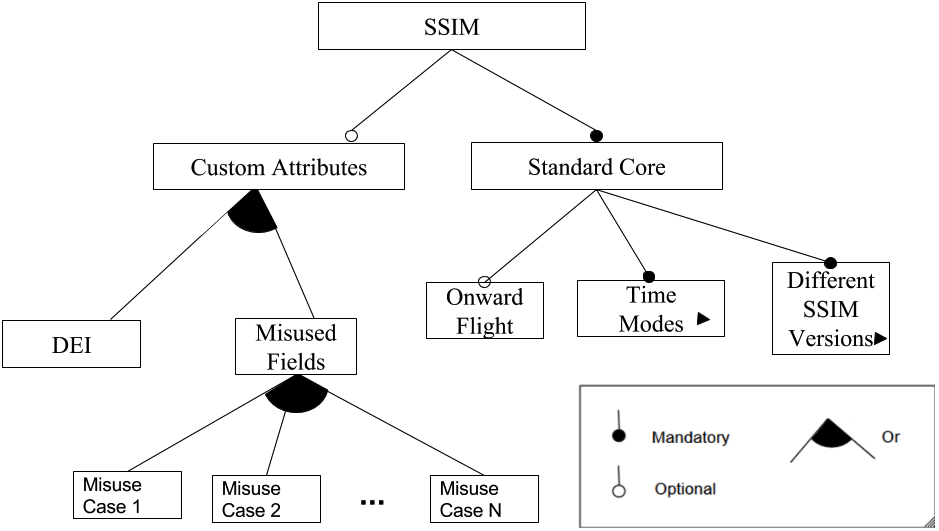
\includegraphics[width=\columnwidth]{figure/figure12.png}

\caption{ Main SSIM variability points using feature diagrams}
\label{fig:SSIMvariability}
\end{figure}



The SSIM standard contains two main parts. The standard core part which contains the fields shared by all the customers.
We found three variation points inside the standard core.
The first one is an optional field for the onward flight information. The second one is the different time modes. Lastly, there can be different versions of SSIM followed by different airlines. We illustrate further the variants of the variation points for the time modes and different SSIM versions in Figure~\ref{fig:SSIM}. %figure 5.2. 

The second part is about extending the standard through custom attributes where the customers can add more functionality.  Custom attributes can take the form of data element identifiers (DEI) which are defined by the IATA manual. They can also take the form of misused fields, where customers violate the syntax in some way.


\begin{figure}[h]
\centering
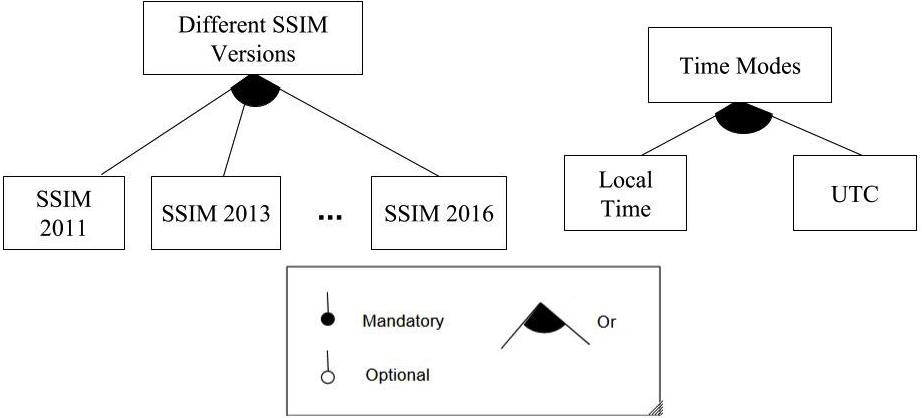
\includegraphics[width=\columnwidth]{figure/figure13.png}
\caption{ Different SSIM Versions and time modes}
\label{fig:SSIM}
\end{figure}



Depending on the IATA manual issue which an airline uses, different SSIM versions can exist. Some airlines might even use very old versions. 
Time modes can be either in Local Time or UTC. In the following sub sections we include more details for each variation point.


\subsubsection{Data element identifiers }
We begin with the Data Element Identifiers (DEI) as the first identified variation point. These can be used to extend the SSIM interface. This way customers can address their individual and distinct needs. DEIs take the form of an integer in a specific field inside the interface. Another string field corresponding to this DEI contains information to address an airlines specific requirements. The DEIs are described by the IATA manual and each integer has a different meaning. Currently there were only four DEIs supported inside the core code of the new system, as their total number can be a few hundred different cases. 


\subsubsection{Misused Fields }
Moreover, there can exist customer specific use cases which can not be handled by the use of DEIs.The system needs to know how it should handle each customer's individual case.  An example of such case is code-share issues, where an airline might wish to replace the subsidiary  carriers with the main carrier. Another example is the departure time shown to the customers and the actual departure time of the aircraft. This might occur because in some airports the passengers are being transported with buses to the aircraft, so there might be a few minutes variation. However, from crew planning perspective the aircraft time is what is important. As a last example, some customers use the flight service type, such as cargo only, in the field that is meant for the flight suffix. Finally, there could exist a case where an airline might want to use a field inside the SSIM interface which is usually not read by Jeppesen's systems. Therefore the system should be aware of this case and act accordingly. 
During the group interview all the stakeholders agreed this was the most urgent variability point.



\subsubsection{Different SSIM versions}
In addition to the custom attributes, different SSIM versions exist. The IATA standard releases a new version of their manual twice a year. During our investigation we used the 2011 version as a reference. Airlines whose systems use a very old version might not be compatible with the newer ones. Throughout the different versions, lots of fields have new meanings. Some unused or empty fields start being used. Some of the fields that the company normally does not read might be required by some customers. However, according to some interviewees in the group interview, this is  rarely a problem as it is very rarely changed in a major way. Furthermore, some clients might have a completely new use case which results on a modified version of the SSIM standard.    

\subsubsection{Time modes }
Another issue is related with the time mode an airline company is using. More precisely, for the date of operation of each flight leg can be specified either in UTC or in Local Time. Although the IATA standard states that the time shall be in UTC, some customers still might want to store it in local time because this was the time format their systems were using. It should be noted that the handling of this issue is responsible for a significant percentage of the old system's code complexity, according to engineers in the company. As an example, a flight from an American airport can take place late at night. If the airline company sends the time in Local Time, the day of operation is different in UTC time because it is a different day in Europe. This can cause confusion, especially since the day of operation for each flight should be unique according to the IATA standard.

\subsubsection{Onward flight}
Finally, stakeholders raised the issue of an optional field containing information about the onward flights. These flights are concerned with the next leg flown by the same aircraft. The information about these flights can either be missing, or it can be included and still not be consistent. The system should be able to handle these cases as this information is necessary for planning purposes. 





\subsubsection{Main variation points of Operational messages interface }
We identified four variation points for the operational messages interface. 
The first variation point is concerned with whether or not the aircraft rotations need to be updated.  Different airlines have different scheduling process. In this interface, the company can choose to either update the onward aircraft rotations by performing an action or keep the same information provided by the SSIM. If the airline actually wishes to update the onward information, functions which swap flight legs or assigning new pointers in the rotations can be called. 

The next variation point is about the time mode for the date of origin. The manual for the operational messages says the time should be in UTC, but some airlines especially in America still use local date of origin because it is easier to keep unique. However, the time obtained from the SSIM interface can still be in Local Time. As an example, a flight starting late at night in USA which uses Local Time, appears to be the next day in Europe. The system therefore needs to know how to properly adjust the date accordingly. 

Another variation point is about the diversions from original schedule. When a flight leg can not land to the original arrival station it might have to land to another airport. This can occur, for example, because of harsh weather conditions. The follow up messages might be different between airlines. The aircraft might have to go back to its original destination, or continue to the next destination. The variation lies on the assumption of what the aircraft should do, as long as not further message arrives or opposite, for what situation additional messages are expected

Finally, the last identified variation point is concerned with the reliability of the different sources the system gets messages from. If an airline company has an internal consolidation system, then this requirement is not needed at all. An example of different sources reliability would be the messages for the actual and estimated time of departure. For actual time of departure the system would typically trust more the messages sent from the aircraft, while for estimated messages it would trust those sent from the airport.  




%\subsection{The old and the new system}
%In this section we present the difference between the old and the new system for when it comes to parse SSIM files. 
%
%\subsubsection{The old system}
%The variability binding takes different approaches in the two systems. The old system provides a form that allows its users to define many parameters when they wish to import the raw data from SSIM files, giving them the capability to configure the system in run time. These parameters correspond to one more flags of the tool. Some of them are taken from the input form, some are taken from the configuration files. The files are then converted to a specified format and handled by the same component of the tool.
%
%The original code, which was written in C language, was closely following the IATA format and it was expected to be used in the same way by all the customers. In reality, the algorithms had to be adjusted to accommodate more customer specific requirements. 
%%This resulted in an immense main function, with many global variables, that is extremely complex, 
%This resulted in an extremely complex code which was 
%hard to read and manage, as described by the company's experts. Although it works correct and satisfies the expected functional requirements, it is hard to maintain as there is a high risk of problems occurring when the system is updated.
%
%\subsubsection{The new system}
%The new system divides the work of interpretation and logic handling between the adaptor and the back end, as shown in Figure 5.3  
%
%\begin{figure}[h]
%\centering
%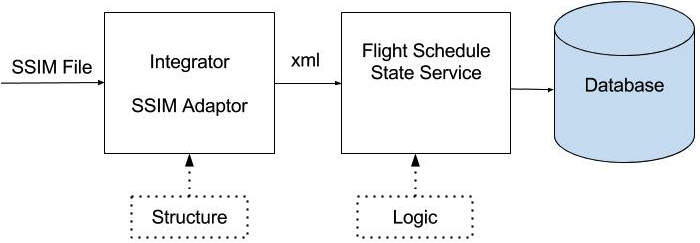
\includegraphics[width=\columnwidth]{figure/Figure2.png}
%
%\caption{ General overview of parsing an SSIM file and storing it in the database}
%\end{figure}
%
%
%The aim is to have separation of concerns between these two components. The SSIM file is generated by an airline company and used as an input to the integrator. The integrator, consecutively, uses an adaptor to define the structure for the SSIM standard in XML form. The ?Flight Schedule State Service? component imports this XML file and applies some well defined computations to handle the given semantics accordingly. Finally it stores in the database the converted information. 
%
%The integrator's code of the new system was originally written in Java. However, during our analysis phase, the company changed the programming language to Python. Although the logic stayed somewhat the same, we had to perform additional code analysis and change our documentation appropriately. For example, the class diagrams had to be redrawn. Based on these diagrams we later placed our proposed solution.\\ 
%An important aspect of our decision making was, for each variability point, which of these two components had to be selected. Whether or not it was a structural or logical problem. 
%Finally, it should be mentioned that the old system is managing variability in run time while in the new system the variability is bound in build time. This means, the old system allows the users to change the interpretation of the parsing of SSIM files by providing an input form containing a number of parameters. However, the new system was initially designed and built to manage customer specific use cases. Later, when they changed the technology from Java to Python, they still provided plug-in scripts which extent the system's core architecture that address customer specific issues. 
%\raggedbottom

\subsection{Indicators for selecting a method}\label{sec:indicators}

There is a number of indicators that greatly influences our decision making for selecting one of the available methodologies. We tried to suggest a way to handle each variation point independently. The first step to manage each of these, according to the guidelines provided by the taxonomy of~\cite{JillesVanGurp2001}, %(Svahnberg, van Gurp \& Bosch, 2005 p708), 
is to identify the variability and where it is needed. These are the variation points which we identified during the context's analysis phase. 

The next step, based on these guidelines, is to constrain the variability. A variation point which can include a significant number of possible alternatives, is often preferable not to include all of them in the first version of the system. The system should include those that are more likely to appear and allow the possibility to accommodate more in the future~\cite{JillesVanGurp2001}. % (Svahnberg, van Gurp \& Bosch, 2005 p710).  

Additionally, the current architecture plays a significant role to our decision making, as there is currently a single fully-working instance of the system. There is a separation of concerns between the parsing of the data and the actual logic handler. We therefore need to decide, for each variability point, which component should we use for our implementation. The technology of the system also is taken into consideration along with its strengths and limitations.

The next step, according to~\cite{JillesVanGurp2001} % (Svahnberg, van Gurp \& Bosch, 2005 p714) 
is to populate the variant feature, that is, how the variant should be created and integrated inside the existing components of the system. The population can either be implicit or explicit. Implicit population means the system does not recognize the available variants. Explicit population means the system actually provides functionality to support the required variants. As an example taken from the authors of the taxonomy, an \textit{IF-Statement} is implicit population, since the system can not usually add more \textit{ELSE-Statements} during run time. This decision indicates when should the binding time of the variants be done. This can either be in build or run time.

In the old system, some of the variants were supported during run time system. The users were able to select the variants they wish during the system's operation through the provided input form when they were loading the SSIM files. There was also a build time option where users could parse a configuration file along with the SSIM files to specify their additional requirements. These files included code which corresponded to the DEIs, as specified in the IATA manual.
In the case of the new system though, the engineers prefer a build time solution. However, run time variability might be supported in the future for some of the variation points. 

Another very important factor is the decision of who is expected to populate a variant feature by writing or compiling code~\cite{JillesVanGurp2001}. % (Svahnberg, van Gurp \& Bosch, 2005 p715). 
The end users can still make use of the customization layer to write their own scripts.
After all, Jeppesen allows their customers to customize their system according to their needs through domain specific language and by Python scripts. As mentioned before, the customers are able to customize the system on the customization layer. For compiling and building the system, it is up to the engineers of the company.

Finally, a decision should be taken of how to bind the variants. This can either be done internally or externally~\cite{JillesVanGurp2001}. % (Svahnberg, van Gurp \& Bosch, 2005 p717). 
Internal binding means that the system provides the required functionality for a particular variation point. External binding means the system makes use of an external entity that implements the binding, such as an external module, another system, an external tool or even a person.


\subsubsection*{Summary of indicators}

\pat{requirements for the solution} The indicators are based on the feedback of the engineers of the new system during the analysis phase of our study. 

Below we present the summary of the indicators:\\

\begin{itemize}



\item The collection of variants should be populated \textit{implicitly}. The company does not wish to include or maintain customer specific code. Therefore, the system needs to include code to only satisfy a particular customer's use cases.

\item The system binds the variability during build time, where it is designed and handed over to the customer.

\item When it comes to who needs to write the required code, the customers are expected to modify the system to handle their variability needs in the form of Python scripts.

\item This means that the functionality should be bounded \textit{externally}. 


\end{itemize}




\section{Development and implementation of proposed solution}

In order to explain the idea of our solution we developed a prototype. 
%The aim of our study is to create knowledge by attempting to solve a concrete customization problem. %In this way, we tried to answer the second research question, that is, in which way we could increase the system's customizability. 
%We proceeded to develop a prototype so as to show the idea. 
We started with the custom attributes variation point, which was considered as the most urgent from the company's stakeholders. 
In this section we present the steps we followed during the development phase of our study. %The discussion of the feedback is described in the next chapter.


%\subsection{Java implementation}
%The integrator's code was initially entirely written in Java. Since there was only one customer, there were not any known customer specific requirements for the new system. Our initial assumption was that the system would require run time binding, because this was the way it worked in the old system. Based on the taxonomy of (Svahnberg, van Gurp \& Bosch, 2005 p735-737) and the figure 5.5
%we considered two code-level realization techniques. The first one was run time variant component specializations and the second was variant component implementations. These techniques make use of design patterns in code level to manage variability. The reason we choose these techniques was based on the indicators which stated that the binding should be done in run time, the collection of variants should be explicit while the system provides internal functionality. 
%
%Our original suggestion was to apply behavioural design patterns. Behavioural patterns are linked with the assignment of responsibilities between objects and the handling of diverse algorithms. These patterns favour object composition over inheritance (Gamma et al. 1995 p221).
%
%For the case of custom attributes, we tried to to make use of the strategy pattern. As originally presented in (Gamma et al. 1995 p315), this pattern defines a family of algorithms, encapsulates each one and makes them interchangeable. Strategy lets the algorithm to vary independently from the clients that use it. In this way we expected that we could encapsulate the required behaviours for the different misuse cases inside separate classes.
%
%We tried to design the parser in a way to make use of this pattern by creating sub-classes. These sub-classes would include the different algorithms for managing the different misuse cases. In this way, we tried to separate the parts of the application that vary and the parts that belong to the core of the product, that need to stay the same. We consider the handling of customer specific use cases as different algorithms that affect the behaviour of the system.
%
%Our assumption was that not many misused cases would appear since this was the general impression we obtained during the group interview. Otherwise, should their number become too big it could lead to class explosion, resulting in increased system complexity. 
%
%
%
%
%\subsection{Change of technology}
%
%The company changed the programming language of the integrator from Java to Python. This was done in order to handle the parsing of multiple SSIM files at the same time. This functionality was also present in the old system. 
%\\
%There is now a main core application written in Java. This application calls python scripts which support the translation of the SSIM input to XML. Furthermore, the company provides customer specific scripts. These scripts inherit and overwrite parts of the core implementation. This way they adjust the system to adhere to each of their customer requirements. The customers can also edit these scripts since there is no need to recompile the system. 

\subsection{Existing solution} %Code analysis results }
%The main logic stays somewhat the same with the Java approach. 
The core of the integrator uses python modules to define the structure and the general parsing rules. The module is called \textit{ssim.py} which is included in the \textit{std\textunderscore interfaces \textunderscore adaptors} core package.

As shown in Figure~\ref{fig:classDiagram}, there is a distinction between the core and customer specific layer. The core part, which is on the right of the figure, handles the generic issues of transforming the SSIM into an xml file. The left part includes scripts which handle the concrete issues that are specific for a specific airline company. The DEIs are handled inside the \textit{ssim.py} inside the package \textit{std\textunderscore interfaces \textunderscore adaptors} of the core part. The IF-statement which handles the data element identifiers is relatively small when our research was performed but it could still significantly increase in size in the future.

The airline specific module \textit{ssim.py} is included inside the \textit{as\textunderscore adaptors} package of the customer specific layer. The script inherits and overwrites parts of the super class it adheres to, without the use of interfaces or abstract classes. The size of this script is limited to less than fifty lines of code and handles two concrete use cases. 
This approach binds the variability in build time. There is clear separation between the core and varying customer specific solutions. In this way, the company increases the maintenance of the system since only the additional scripts need to be maintained which cause no ripple effects to other modules. 


\begin{figure*}[h]
\centering
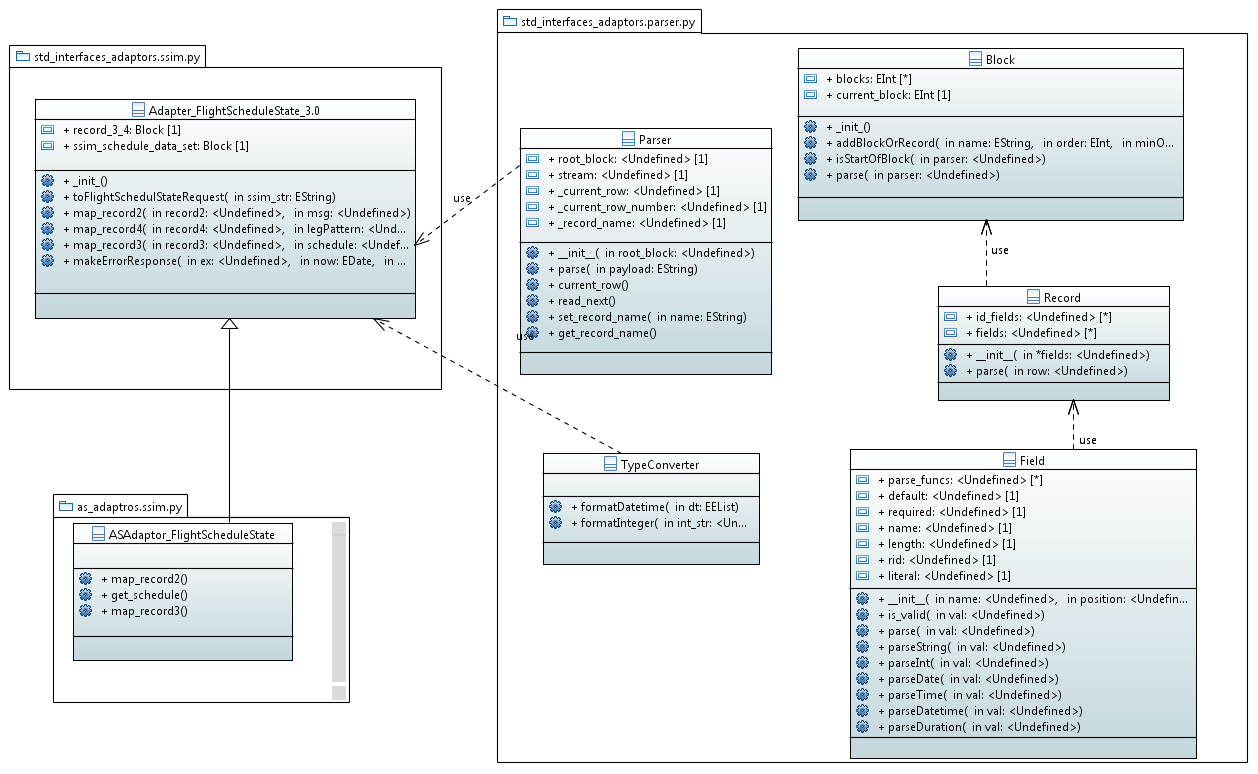
\includegraphics[width=1.0 \textwidth]{figure/figure8.png}

\caption{Existing solution}
\label{fig:classDiagram}
\end{figure*}


\subsubsection{Issues of the existing solution}

The approach the company is following is quite efficient. The core stays the same for all customers and they are responsible for editing scripts to customize it further. They are also responsible for their maintenance and keep it compatible with their systems; Jeppesen loses control over the code. 

During our study we raised some issues. Hard-coded conditions were included inside the customer specific scripts. The follow-up question was whether or not we could somehow reuse parts of the code. In this way, we hoped to decrease the amount of code required to handle use cases which appear more than once.


Another issue we raised was to what extent could the airlines write quality code by themselves. After all, they need to focus on airline related problems than programming related problems. Writing a Python script requires understanding of the system's core code as well as writing test cases to ensure the code provides the expected results.


Finally, there was the issue concerning what would happen when all the company's customers migrate to the new system. The maintenance is done by the airlines side which means they are responsible to keep compatible their systems. 
According to some stakeholders who come in contact with customers, they receive support calls when their customers can not figure out how to fix their systems and even sometimes they complain that they receive too much code to maintain.  

By the time this study was performed, there was only one airline supported in the new platform and the company was talking with the second customer. The goal of this study was to look further ahead and suggest a way to mitigate emerging risks.  

\subsubsection{Suggested approach}
%Contrary to our initial approach, we decided our method should 
Our approach aims for build time binding and implicit collection of variants and external functionality. This decision was made by asking some practitioners within the company whether run time binding was needed. %This question was asked to the developers of the new system after the Java-to-Python transition was made. 

Based on the \todo{above indicators}, we looked into different techniques of the taxonomy, such as the variant component specializations and optional component specializations~\cite{JillesVanGurp2001}: % \todo{(Svahnberg, van Gurp \& Bosch, 2005 p733-735)}: %These choices follow the figure 5.5. and based on the indicators we discussed in section 5.3, we selected two methods as follows:

 \begin{figure*}[!t]
 \centering
 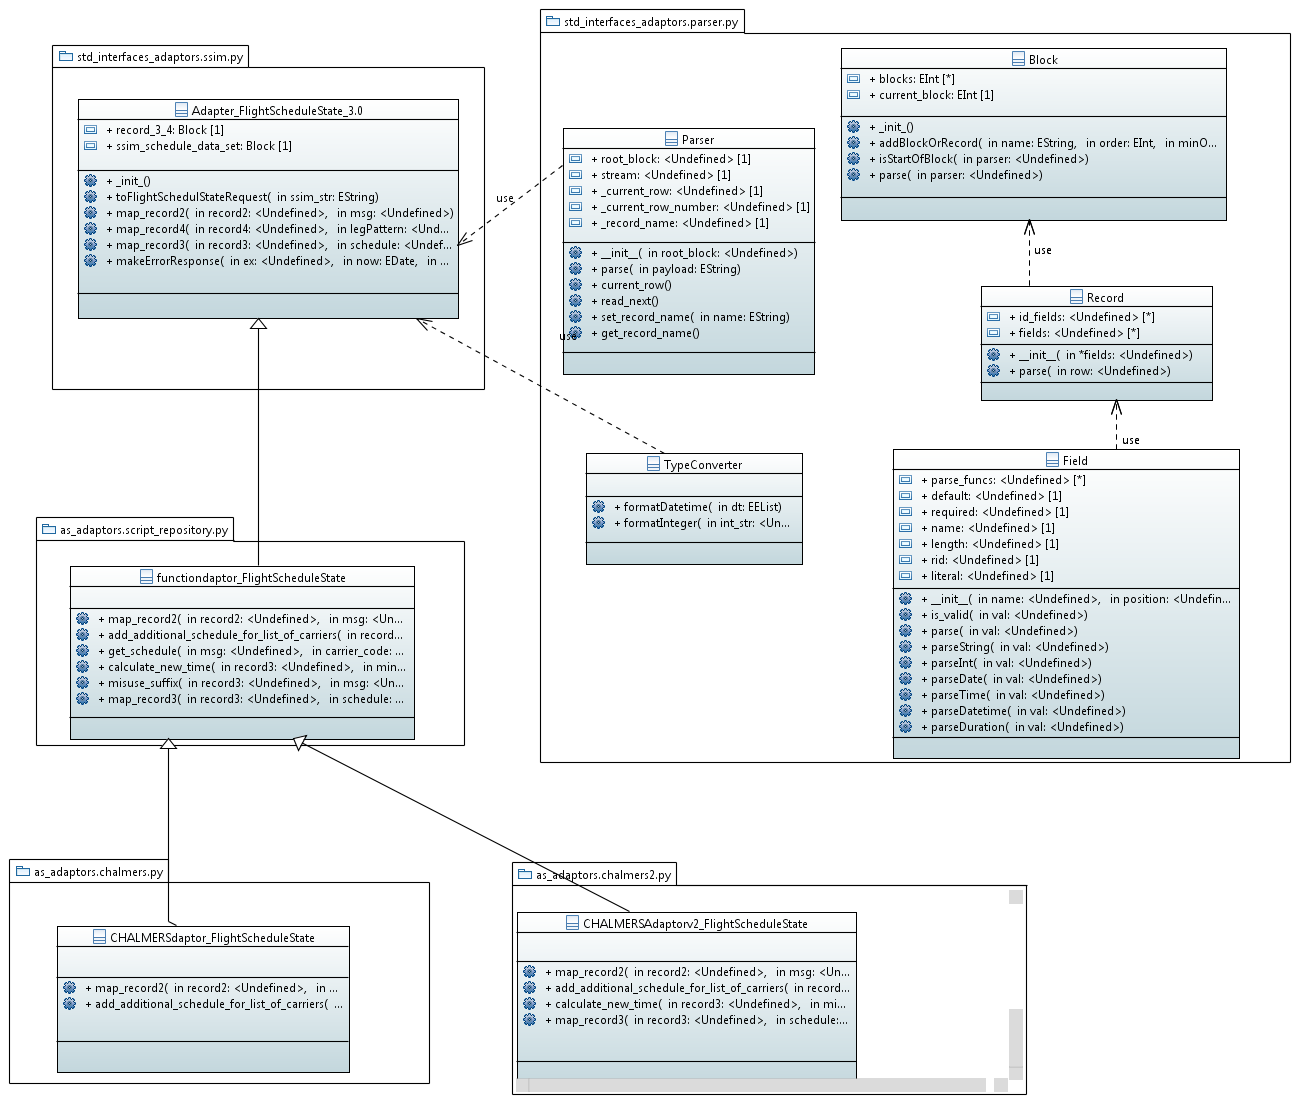
\includegraphics[width=1.0 \textwidth]{figure/figure9.png}
 
 \caption{Approach using a script repository in Python}
 \label{fig:ourApproach}
 \end{figure*}


\textit{Variant component specializations} suggest a method where a particular component is adjusted to addresses different variability issues. This is realized by creating a number of independent classes and selecting those who are required to be included for each case. 

\textit{Optional component specializations} is about including or excluding the relevant behaviour of a component for each case. This can be realized by developing a separate class which encapsulates the optional behavior~\cite{JillesVanGurp2001}. % \todo{(Svahnberg, van Gurp \& Bosch, 2005 p733-735)}.
 

Inspired by those methods, our new approach suggested a grouping of the recurring methods in a separate module. This module would inherit and overwrite parts from the core implementation but the customers would only need to import this module on their scripts and use the available methods by simply parsing parameters. 

The main idea was to support the customization by allowing the users to select among a set of provided functions instead of customizing those functions.
In this way, we hoped to reduce the code duplication for handling these case as we expect that only the provided parameters will change in the future. We also hoped we would increase the understandability of the system. 

\subsection{Development process}
To achieve this, we developed a new Python module which contains methods to handle misuse cases. We called this python module as \textit{script\textunderscore repository.py} and we created two children scripts, \textit{chalmers.py} and \textit{chalmers2.py} that made use of the provided scripts to handle a number of concrete use cases. In Figure~\ref{fig:ourApproach} we present the class diagram of our approach.






In order for the script repository to define algorithms for each use case, different parts of the core implementation had to be taken into consideration, such as the provided methods and data structure definitions. 


Our prototype's was built in a test driven development approach; we first wrote a test case, we let it fail and we proceeded to write code to make it pass. For this reason, we have written a new file explicitly for writing our own test cases which were satisfied by the modules  \textit{chalmers.py} and \textit{chalmers2.py}. Moreover, we have written a test case that only makes use of the core implementation in order to make sure we have not altered anything in this part and that the core is working as expected. 

The \textit{script\textunderscore repository.py} is the module which needs to be maintained and extended. The children modules only needed to call these methods and provide the appropriate parameters. 

\subsubsection{Example use cases}
To show the idea behind our approach, we tried to support a few use case. Two of these use cases were making use of a certain airline's requirements, which the engineers have solved but in a hard-coded way. These use cases were related with replacing the codes of the subsidiary carriers to to the main carrier and the inclusion of additional schedules to these subsidiary carriers. Our approach would only require the customer to import our module and call these methods with the corresponding parameters.

We also tried to solve some conceptualized use cases, based on what we discovered during our interviews in the analysis phase.
The first use case had to deal with the time variation of the departure time. If the departure time had to be adjusted a few minutes, the script would again only require to import our repository and call the corresponding method with the appropriate parameters. 
Finally, we tried to handle the misplacement of the service type suffix, when some airlines use the operational suffix instead of service type field. We handled this case in the similar fashion as above, by calling the corresponding method. In this case, however, no parameters were required.

Our approach follows our initial assumption that not too many customer specific requirements would emerge. Should this be the case, there could be an explosion of methods. Additionally, these methods are only viable if they are required from at least more than one customer. In the next chapter we provide a more detail discussion about this approach. 


\subsubsection{The rest of the variation points} 
We have observed that not all of the issues can be handled with the same method. For each individual variation point a decision had to be made on which part of the system it should be handled. More precisely, for each variation point we had to decide whether it could be solved as a structure or logic issue. Therefore, the adapter or the logic-handler modules would had to be selected respectively. 

The focal point of was placed mostly on the different misuse cases. We have investigated further of how to handle the rest of the variation points to decide whether or not it could be handled with our approach or in a different way. Our findings suggest that not all points could be handled with our suggestion. 

Local time and UTC time adjustments require special logic handling. The algorithms responsible for this handling have already implemented in the logic component of the new system. The only requirement is that the input XML file provides the correct semantics to define whether the time is Local Time or UTC time. In this way, there is no need to adjust the system for each customer as it is able to handle all cases.

Similarly, the onward flight has been handled in this way. The algorithms to handle inconsistent or missing onward information is handled for all customers in the same way inside the logic part of the system. According to company's experts, there could still be a way to provide a generic method to handle this issue. However, the required parameters would probably be too many and the time needed to investigate how this could be implemented would probably be immense. We therefore decided that this variation point is out of the scope of our thesis.

We have verified that the DEIs are being effectively handled in the core part of the system. After all, DEIs follow are defined by IATA standard and do not misuse the SSIM syntax. We have validated this functionality by writing tests and compare the expected output with a given input based on SSIM files we obtained from the company. 

For special cases of certain DEI numbers, an IF-Statement in the core part suffices. This method is also described in the taxonomy of~\cite{JillesVanGurp2001} %\todo{(Svahnberg, Gurp, Bosch 2005 p739)} 
as \textit{Condition on variable} which intent is to include functionality to support multiple operations. There are currently only a small subset of all the possible integers a DEI can have, as not all of them are required by all the customers right now. For each new customer who actually wants to use a new DEI, a new ELSE-Statement would be added. Therefore the overall IF-Statement could become potentially big and since it is currently included in the core part of the parser, it would might add up to its complexity. If this should be the case, we suggest to include this IF-Statement into a separate module and call it through the main core implementation by parsing the corresponding DEI. 


Finally, when it came to handle the different versions of the SSIM interface, we observed that this could be handled in a similar way as with the misuse cases. If there are major differences between the supported version and the version an airline is using, it is implied that there is a need for adjustment. Company's experts have also agreed that this case could be considered as a special case of syntax misuse.
As an example, a field of an older version could have a different meaning than the current version. Should this be the case, then a method from our repository could be called and adjust the system in the appropriate way. 

However, during our investigation we have observed that if a customer wants the system to read a field that the company usually does not support, this can not be simply handled with our approach. We tried to write a method to handle this issue but it was futile as the system would require to be rebuilt and recompiled to become aware of this field. Our conclusion, supported by the developers of the new system, was that this can only be solved manually by the company's side.


\subsubsection{Operational messages variation points} 

We tried to discuss ways to deal with the variation points of the operational messages interface. The suggestions include high-level methods to handle variability in this context. The aim to see whether or not the suggestions made for the SSIM interface could be replicated in this context. The discussion involved the system architect of the new system. Evaluation of this discussion was performed during the last presentation in the company which also involved engineers of the new system. Everyone seemed to agree with these suggestions. We assume that the company would follow the same logic of separation of concerns, where the raw input is translated to XML semantics and is being handled in the backend. 

For the updated aircraft rotations variation point, there is a need to indicate whether or not the flight legs need to be updated. The decision whether or not to update these rotations could therefore be considered as a structural issue. Depending on an indicator, the corresponding function could be called.  
By default it would assume that there is no need to update the rotations at all. The functions would be written by Jeppesen engineers but the selection could be done by the customers. Therefore the algorithms could be part of the core and encapsulated in the backend. The customers could simply edit a script to include an indicator to call these functions.

In a similar fashion the date of origin could be managed. A flag in the translated xml file could indicate that a system is using local time. The recalculation is done in the backend part of the core. Therefore it is shared among all customers and the functions are written by the company's engineers. The selection among the functions could simply be done by the customers. 

The reliability of the different priorities is a rather complex variation point. It could be done entirely in the customization layer and it would require explicit functions which would overwrite parts of the core. The system could prepare support for priority handling, either in the core or in the customization layer.

Finally, the diversions variation point could be viewed as a structural issue. The point is to define which would be the next flight leg. This could be handled by editing a script and calling the corresponding function and parsing parameters. This is intertwined with the repository of scripts suggestion of this study. However, if the functions are proven to be rather hard to replicate because of vast numbers of parameters, documentation and coding standards could facilitate this purpose.